\documentclass[10pt,twocolumn]{scrartcl}

\usepackage[utf8]{inputenc}
\usepackage[T1]{fontenc}
\usepackage[ngerman]{babel}

\usepackage{amsmath}
\usepackage{amssymb}

\usepackage{graphicx}
\usepackage{tabularx}

\setlength{\parindent}{0cm}
\setlength{\parskip}{3mm}
\setlength{\textheight}{23.8cm}
\setlength{\headheight}{1cm}
\setlength{\topmargin}{-10mm}

\setlength{\oddsidemargin}{0cm}
\setlength{\evensidemargin}{0cm}
\setlength{\textwidth}{16cm}
\setlength{\columnsep}{8mm}

\usepackage{multicol}
\usepackage{colortbl}
\usepackage{xcolor}
\definecolor{grau}{gray}{0.95}
\definecolor{dunkelgrau}{gray}{0.85}

\usepackage[normal]{caption}

\setlength{\parindent}{5mm}
\setlength{\parskip}{0mm}

\usepackage{float}
\restylefloat{figure}

\renewcommand{\topfraction}{0.75}
\renewcommand{\textfraction}{0.2}

%###########################################################
% custom
\newcommand{\TITLE}{Evaluation von Intervallschätzungen und Paramtertests\\ am Beispiel des Buffonschen Nadelproblems}
\newcommand{\AUTHORS}{Lukas Rosenbach\\ David Lennart Risch}

\usepackage[
hidelinks, 
linktoc=all
]{hyperref}

\clubpenalty = 10000
\widowpenalty = 10000
\displaywidowpenalty = 10000
%###########################################################

%###########################################################
% die Sachen mit der Kopfzeile
\usepackage{lastpage}
\usepackage{fancyhdr}
\fancyhf{} % leere alle Felder
\fancyhead[R]{\footnotesize \AUTHORS}
\fancyhead[L]{\footnotesize \TITLE} % Titel des Aufsatzes
\fancyfoot[C]{\footnotesize \thepage/\pageref{LastPage}}
% \fancyfoot[C]{\footnotesize \thepage}
\renewcommand{\headrulewidth}{0.4pt} % obere Trennlinie
\pagestyle{fancy}
%###########################################################

\newcommand{\ownsection}[1]{\begin{center}\LARGE\textbf#1\end{center}}

\begin{document}

\twocolumn[
\ownsection{\TITLE}

\begin{center}
\AUTHORS \\
Mannheim, Juni 2020
\end{center}
\vspace*{5mm}
]

\section*{Abstract}

\section*{Einleitung}


\section{Material und Methoden}

	\subsection{Buffonsches Nadelproblem}
		\label{chap_buffon_needle}
		Bei dem Buffonschen Nadelproblem, das erstmals von Buffon im Jahr 1733 behandelt wurde, geht es um die Wahrscheinlichkeit, dass eine Nadel, die auf eine Fläche mit parallelen Linien gleichen Abstands geworfen wird, eine Linie schneidet.
		
		Dieses Experiment beinhaltet eine Nadel der Länge l, die in einem Winkel $\theta$ auf eine Fläche mit parallelen Linien mit dem Abstand d fällt. Für eine kurze Nadel, also l < d, lässt sich die Wahrscheinlichkeit wie folgst berechnen: \cite{MathWorld}
		
		\begin{equation}
			x \equiv \frac{l}{d}
		\end{equation}
		
		\begin{align}
			P(x) &= \int_{0}^{2\pi}\frac{l|\cos{\theta}}{d}\frac{d\theta}{2\pi}\\
			&= \frac{2l}{\pi d}\int_{0}^{2\pi}\cos{\theta}d\theta\\
			&= \frac{2l}{\pi d}\\
			&= \frac{2x}{\pi}
		\end{align}
		
		Für einen Linienabstand von 2l entspricht die Wahrscheinlichkeit $1/\pi$.
		
		\begin{align}
			P &= \frac{2l}{\pi d}\\
			&= \frac{2l}{\pi 2l}\\
			&= \pi
		\end{align}
		
		Somit ist es möglich mithilfe eines Monte-Carlo-Verfahrens den Wert von Pi mit dem Buffonschen Nadelexperiment anzunähern.
		
\section{Konfidenzintervalle}
	\subsection{Überblick}
	\label{chap_sim_results} %todo: real location
	
	Ein Konfidenzintervall ist ein Bereich, in dem ein bestimmter Parameter mit einer bestimmten Wahrscheinlichkeit liegt. In diesem Kapitel werden Konfidenzintervalle für den Mittelwert $\mu$ und die Varianz $\sigma^2$ untersucht. Diese können verwendet werden um Aussagen über einen unbekannten Parameter der Grundgesamtheit aus den Werten einer Stichprobe treffen zu können. In Abbildung \ref{fig_mean_interval_hist} ist das $80\%$ Konfidenzintervall des Mittelwerts dargestellt. In diesem Fall ist das Intervall korrekt, da der wahre Mittelwert, der Hochpunkt der orangen Kurve, innerhalb des Intervalls liegt.
	\begin{figure}[h]%
		\centering
		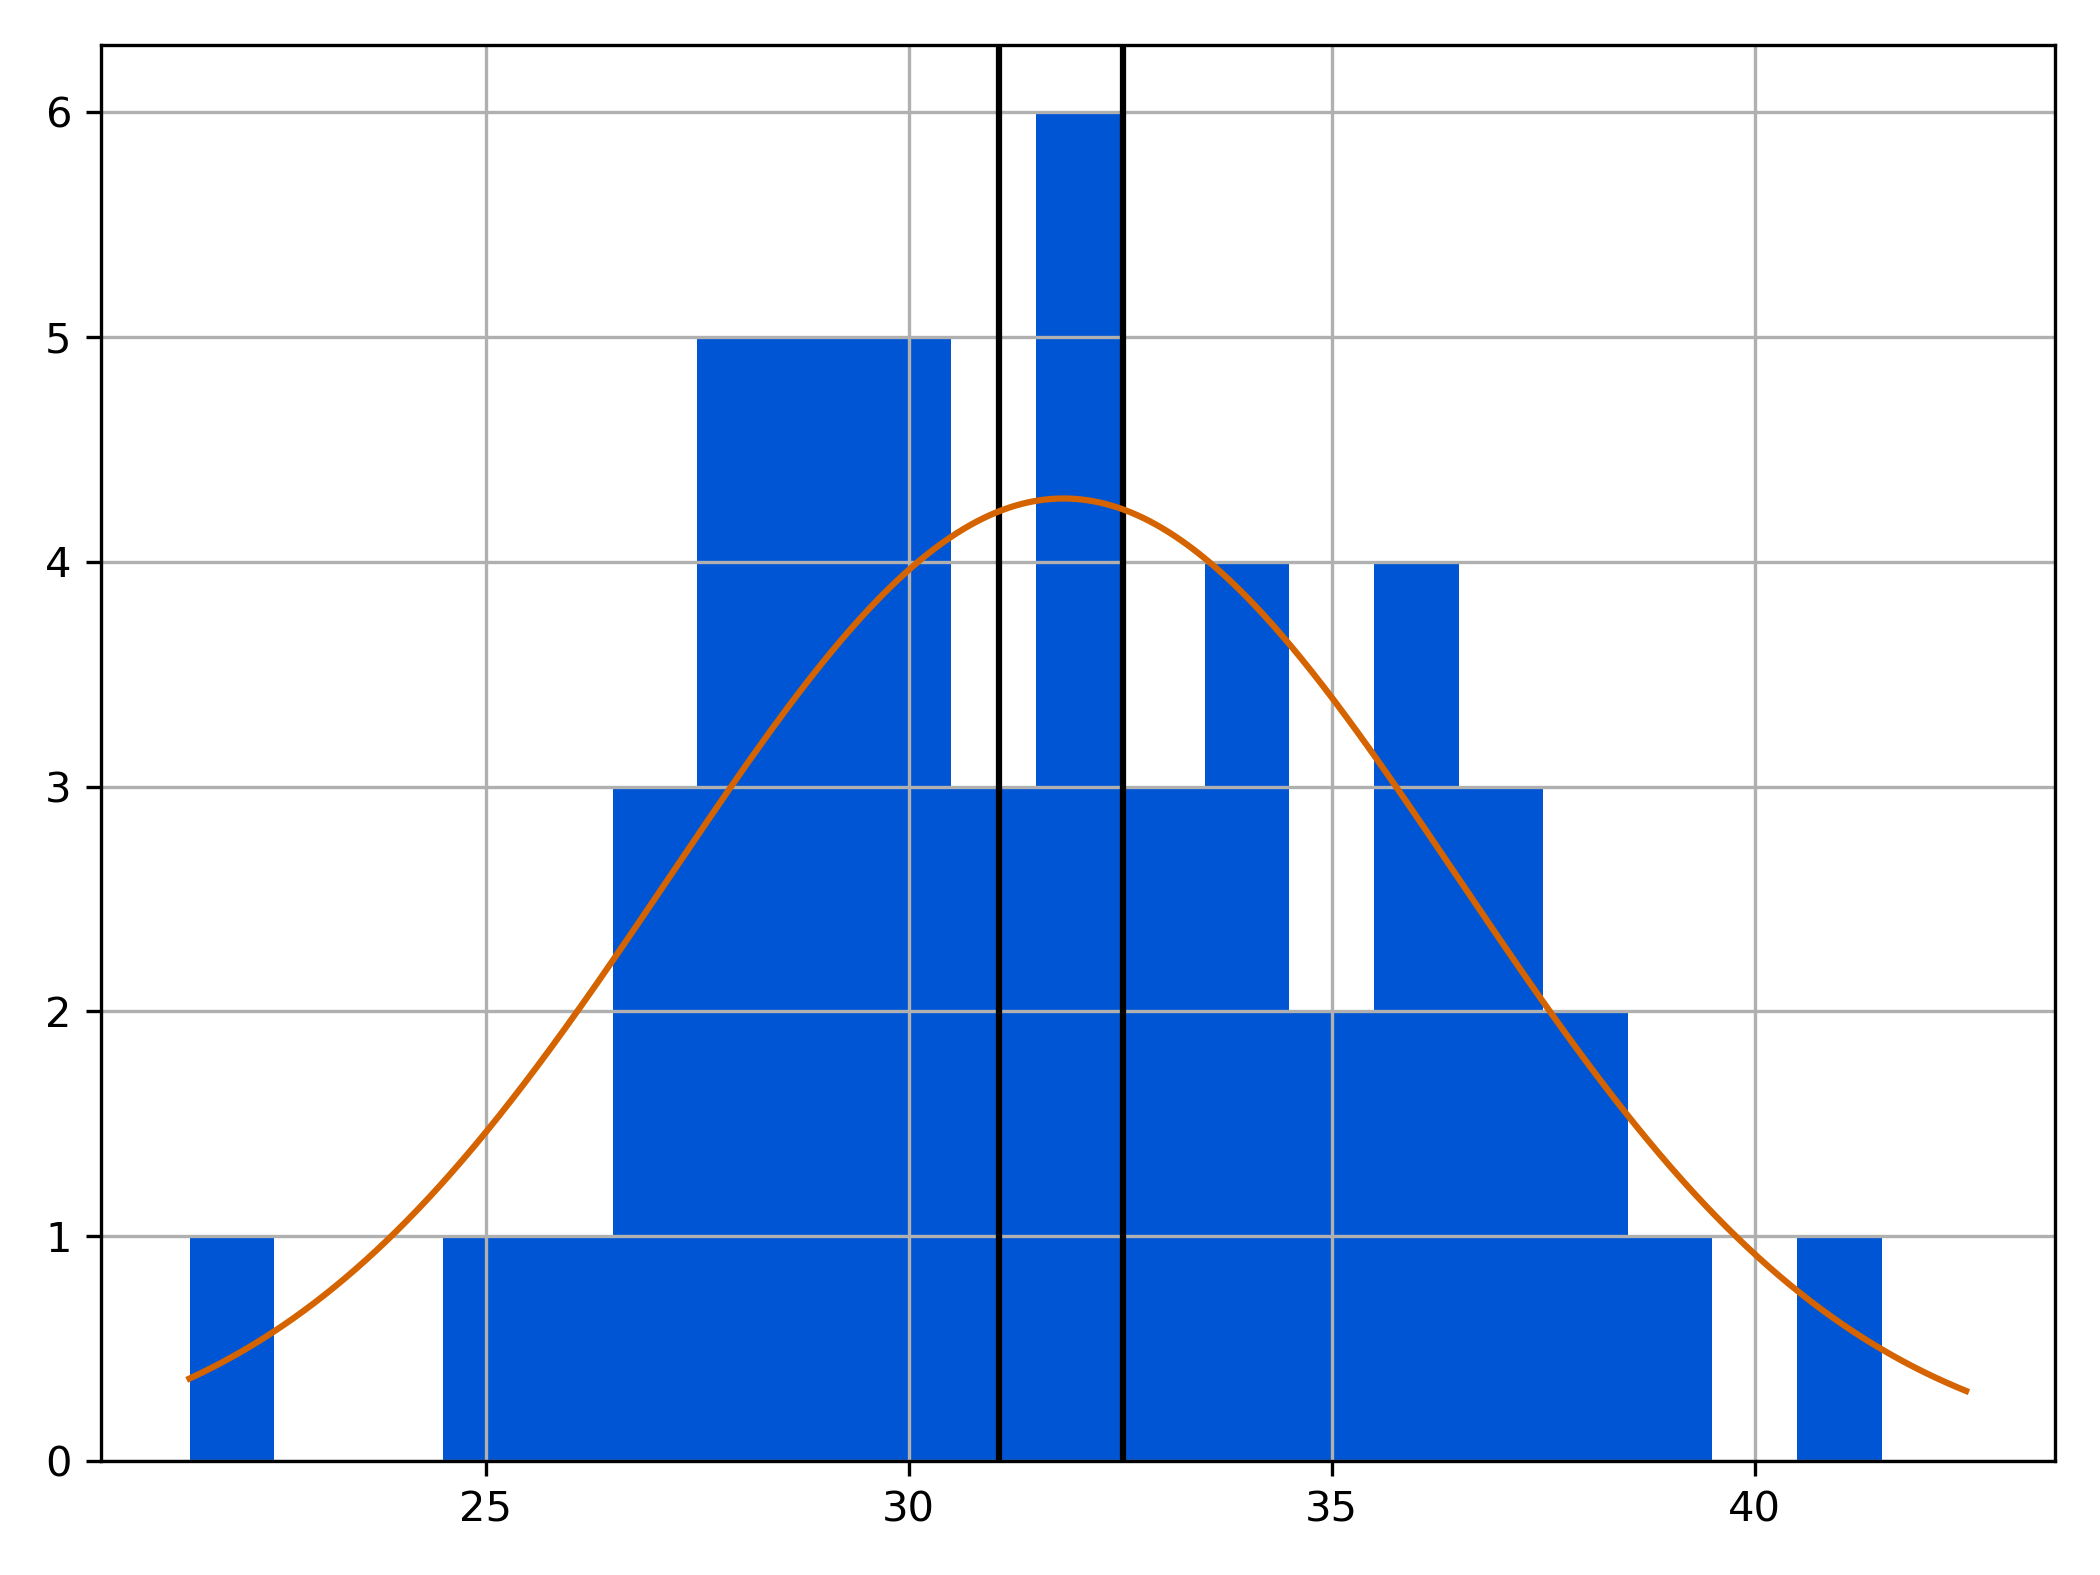
\includegraphics[width=0.9\columnwidth]{images/histogram_50.png}
		\caption{Eine Normalverteilung (orange), $50$ nach dieser Verteilung verteilte Werte (blau) und ein aus diesen berechnetes $80\%$ Konfidenzintervall des Mittelwerts (schwarz)}
		\label{fig_mean_interval_hist}
	\end{figure}
	\subsection{Herleitung des Mittelwerts Konfidenzintervalls}
		\label{chap_interval_mean_math}
		Gegeben sind $n$ Stichprobenwerte $x_1, x_2, ..., x_n$ und ein Konfidenzniveau $\gamma$ bzw. eine Irrtumswahrscheinlichkeit $\alpha = 1 - \gamma$.
		Ziel ist die Bestimmung von $c_1$ und $c_2$ sodass 
		\begin{equation} \label{eq_intervall_norm}
		P(c_1 \le \overline{X} \le c_2) = \gamma
		\end{equation}
		gilt.
		Der Durchschnitt der Stichprobe $\overline{x}$ und die geschätzte Standardabweichung $s$ lasen sich direkt aus den Stichprobenwerten berechnen:
		\begin{align} 
		\overline{x} &=  \frac{1}{n} \sum_1^n{x_i} , \\
		s &= \frac{1}{n-1} \sum_1^n{(x_i - \overline{x})^2} .
		\end{align}
		Um Gleichung \ref{eq_intervall_norm} umformen zu können wird eine weitere Zufallsvariable eingeführt:
		\begin{equation} \label{eq_intervall_t}
		T = \frac{\overline{X} - \mu}{\frac{S}{\sqrt{n}}} .
		\end{equation}
		Gleichung \ref{eq_intervall_norm} kann jetzt mit $T$ umformuliert werden:
		\begin{align}
		\gamma &= P(-c \le T \le c) \\ \nonumber
		\gamma &= P(T \le c) - P(T \le -c) \\ \nonumber
		\gamma &= P(T \le c) - (1 - P(T \le c)) \\ \nonumber
		\gamma &= 1 - 2 P(T \le c) \\
		P(T \le c) &= \frac{\gamma + 1}{2} .
		\end{align}
		Da $P(T \le c)$ dem Quantil einer t-Verteilung mit $N = n-1$ Freiheitsgraden entspricht, kann der Wert von $c$ aus einer Tabelle abgelesen werden. Ein genaueres Ergebnis bietet die Funktion \texttt{scipy.stats.t.ppf(x, N)} der Python Bibliothek scipy.
		Aus der Definition der Zufallsvariable $T$ in Gleichung \ref{eq_intervall_t} ergibt sich für die Grenzen des Intervalls:
		\begin{equation}
		c_1 = \overline{x} - \frac{cs}{\sqrt{n}} \mbox{ und } c_2 = \overline{x} + \frac{cs}{\sqrt{n}}.
		\end{equation}
		
	\subsection{Herleitung des Varianz Konfidenzintervalls}
		\label{chap_interval_var_math}
		Die Herleitung des Varianz Intervalls verläuft analog zu dem Konfidenzintervall  des Mittelwerts. Anstelle einer t-Verteilung wird eine Chi-Quadrat-verteilte Zufallsvariable eingeführt:
		\begin{equation} \label{eq_intervall_z}
		Z = (n-1)\frac{S^2}{\sigma^2} .
		\end{equation}
		\begin{align}
		\gamma &= P(c_1 \le Z \le c_2) \\ 
		\gamma &= P(Z \le c_2) - P(Z \le c_1) \nonumber \\
		P(Z \le c_1) &= \frac{1}{2} (1-\gamma) \\
		P(Z \le c_2) &= \frac{1}{2} (1+\gamma)
		\end{align} 
		$P(T \le c_{1,2})$ entspricht jeweils einem Quantil einer Chi-Quadrat-Verteilung mit $N = n-1$ Freiheitsgraden, dies kann durch \texttt{scipy.stats.chi2.ppf(x, N)} berechnet werden.
		Aus der Definition der Zufallsvariable $Z$ in Gleichung \ref{eq_intervall_z} ergibt sich das Konfidenzintervall der Varianz:
		\begin{equation}
		(n-1)  \frac{s^2}{c_2} \le \sigma^2 \le (n-1)  \frac{s^2}{c_1}.
		\end{equation}
			
	\subsection{Empirischer Beweis}
		Insbesondere durch die Annahmen, die in Gleichung \ref{eq_intervall_t} und \ref{eq_intervall_z} eingeführte  Zufallsvariablen $T$ und $Z$ würde genau einer t-Verteilung bzw. Chi-Quadrat-Verteilung mit jeweils $N = n-1$ Freiheitsgraden entsprechen, ist die Herleitung alleine nur bedingt geeignet um die daraus gewonnen Formeln zu plausibilisieren.
		
		Um die Korrektheit der in Kapitel \ref{chap_interval_mean_math} hergeleiteten Formeln zu bestätigen wurde ein empirischer Beweis durchgeführt. Die Berechnung wurde in Python implementiert und können so beliebig oft mit den in Kapitel \ref{chap_sim_results} erstellten Daten durchgeführt werden.
		
		Der folgende Test wird separat für mehrere Werte von $\gamma \in [0, 1]$ durchgeführt. Es wird für $n = 100$ Werte das Konfidenzintervall des Mittelwerts und der Varianz mit einem Konfidenzniveau $\gamma$ gebildet. Durch den in Kapitel \ref{chap_buffon_needle} hergeleiteten Wert für $p$ können der theoretisch zu erwartenden Mittelwerts und die Varianz berechnet  werden:
		\begin{align}
		E(X) &= n p , \\
		\sigma &= n p (1-p) , \nonumber \\
		Var(X) &= \sigma^2 = (n p (1-p))^2 .
		\end{align}
		
		Es wird überprüft, ob der Erwartungswert und die Varianz innerhalb oder außerhalb des geschätzten Intervalls liegen. Dieser Vorgang wird in $1000$ Durchläufe wiederholt, dabei wird der Anteil an korrekten Intervalle gezählt. Das Verhältnis zwischen $\gamma$ und dem tatsächlichen Anteil an korrekten Intervallen ist in Abbildung \ref{fig_mean_interval_dot} und \ref{fig_var_interval_dot} zu sehen. Dabei liegen Punkte für alle Werte von $\gamma$ auf einer Ursprungsgerade mit Steigung $1$, dies bestätigt die Korrektheit der Formeln zur Berechnung des Intervalls. Die leichten Abweichungen der einzelnen Punkte sind durch die begrenzte Anzahl an Durchläufen und den recht kleinen Stichproben zu erklären.
		
		
		\begin{figure}[H]
			\centering
			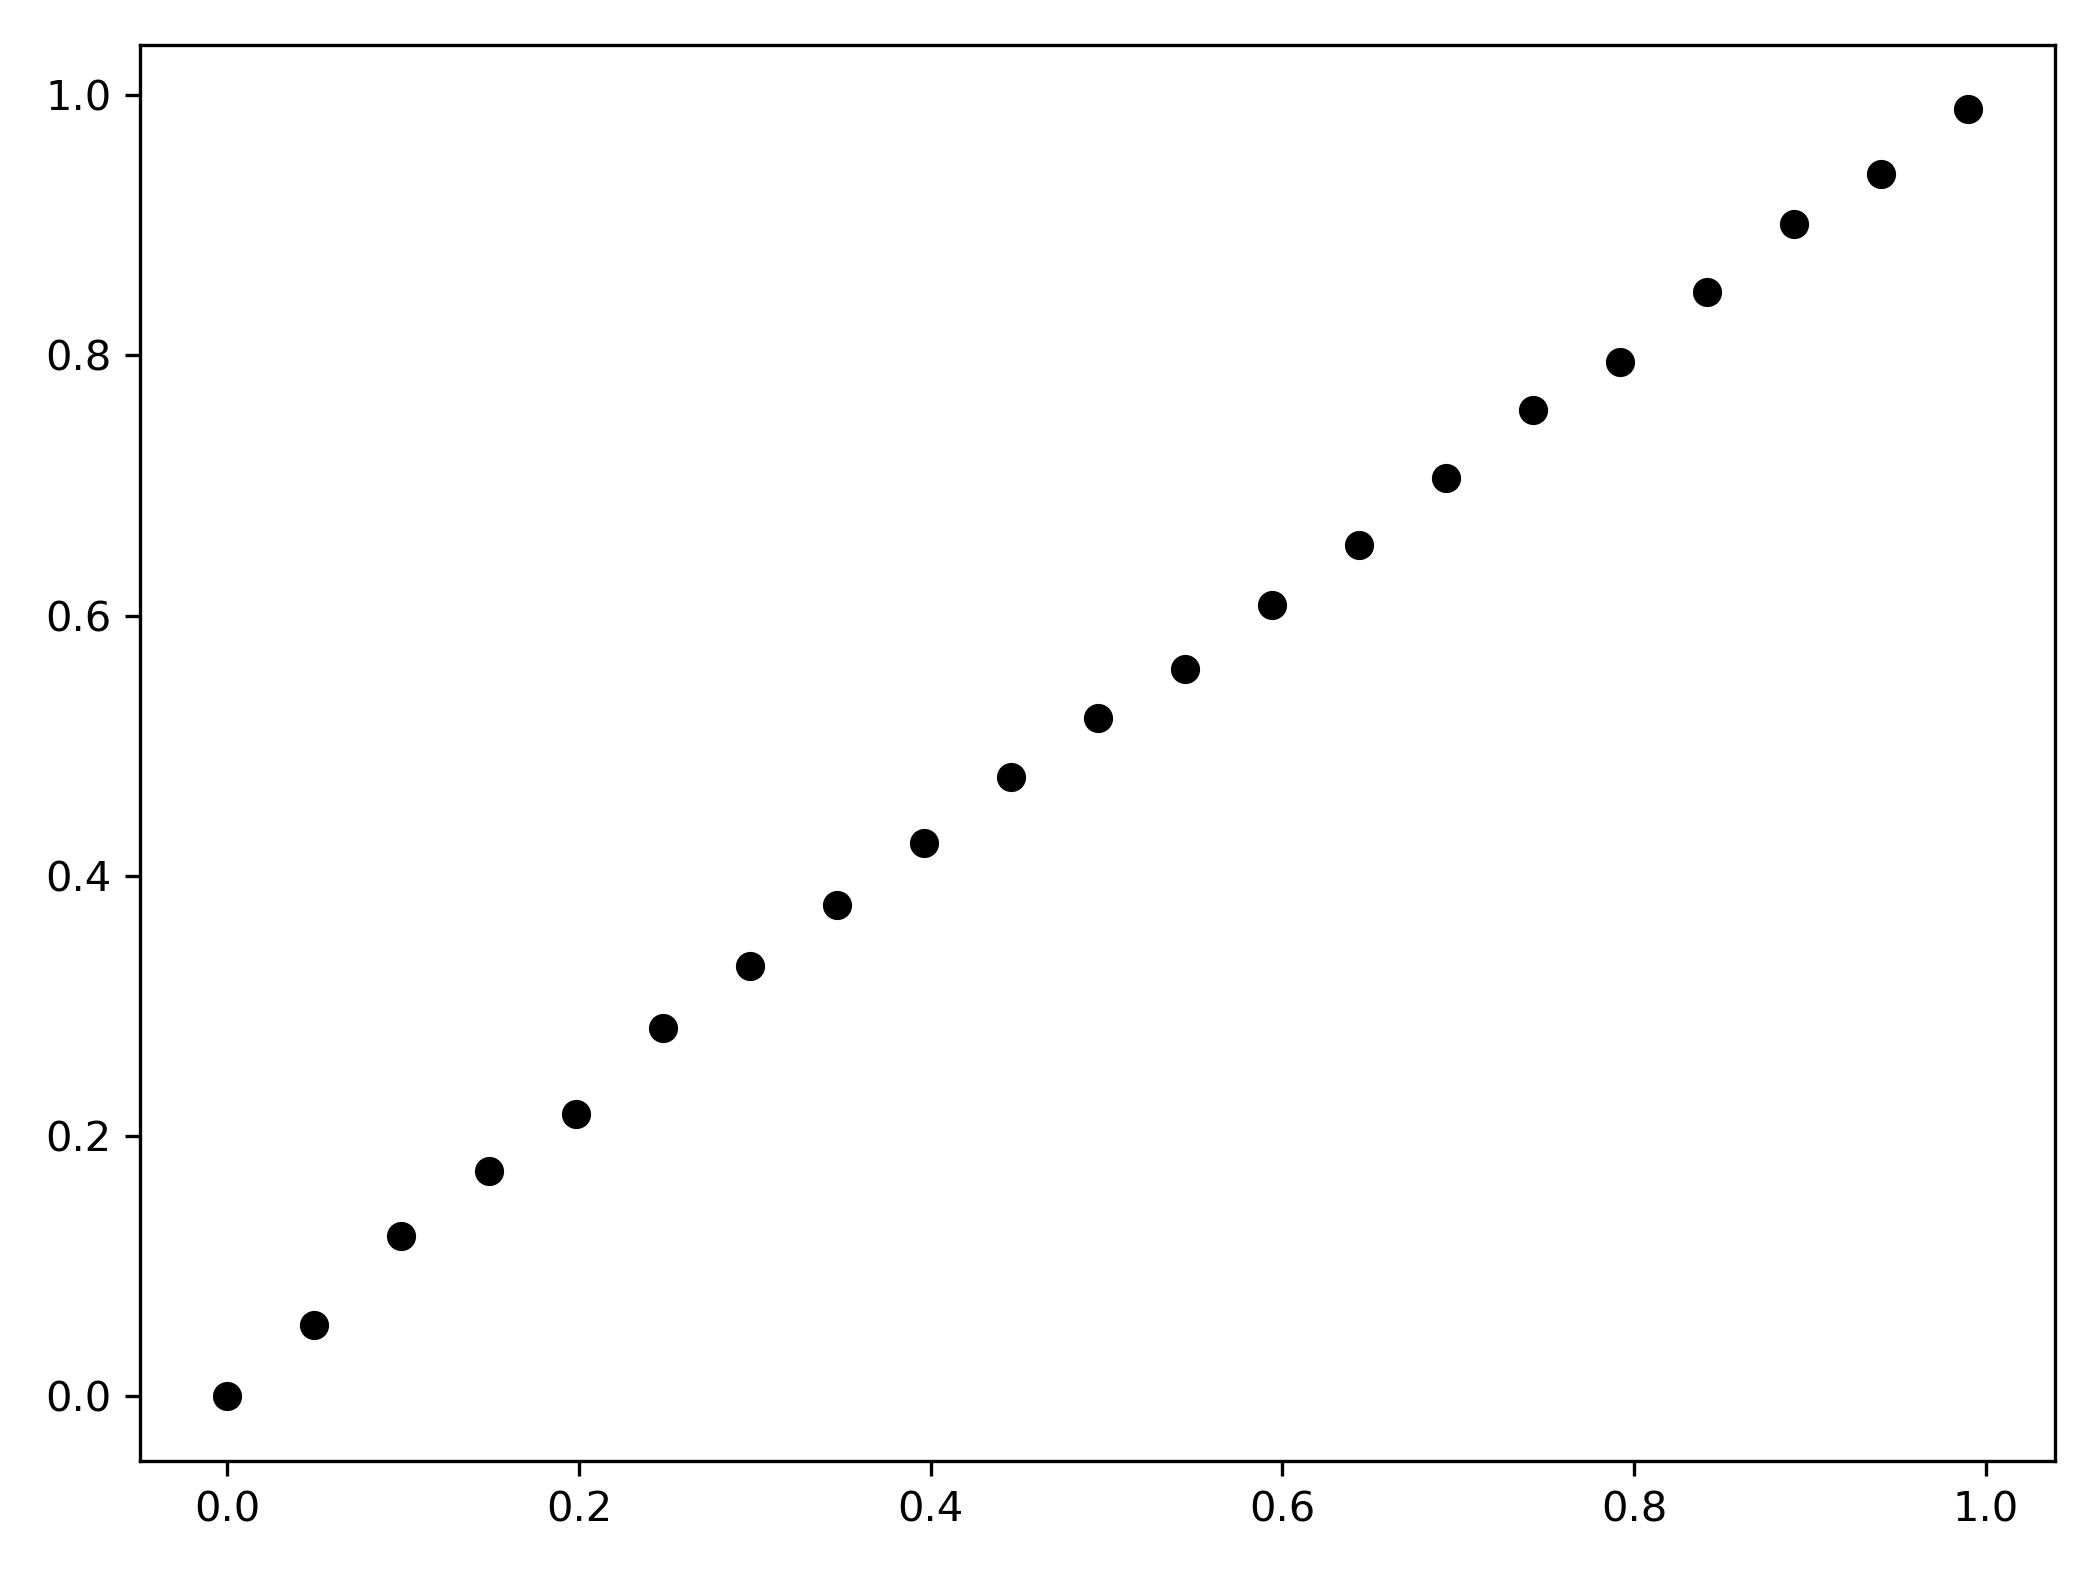
\includegraphics[width=0.9\columnwidth]{images/mean_interval.png}
			\caption{Mittelwerts Intervall: Verhältnis zwischen $\gamma$ (x-Achse) und dem tatsächlichen Anteil an korrekt geschätzten Intervallen (y-Achse) für $1000$ Durchläufe je $\gamma$ mit Stichprobenumfang $100$}
			\label{fig_mean_interval_dot}
		\end{figure}
	
		\begin{figure}[H]
			\centering
			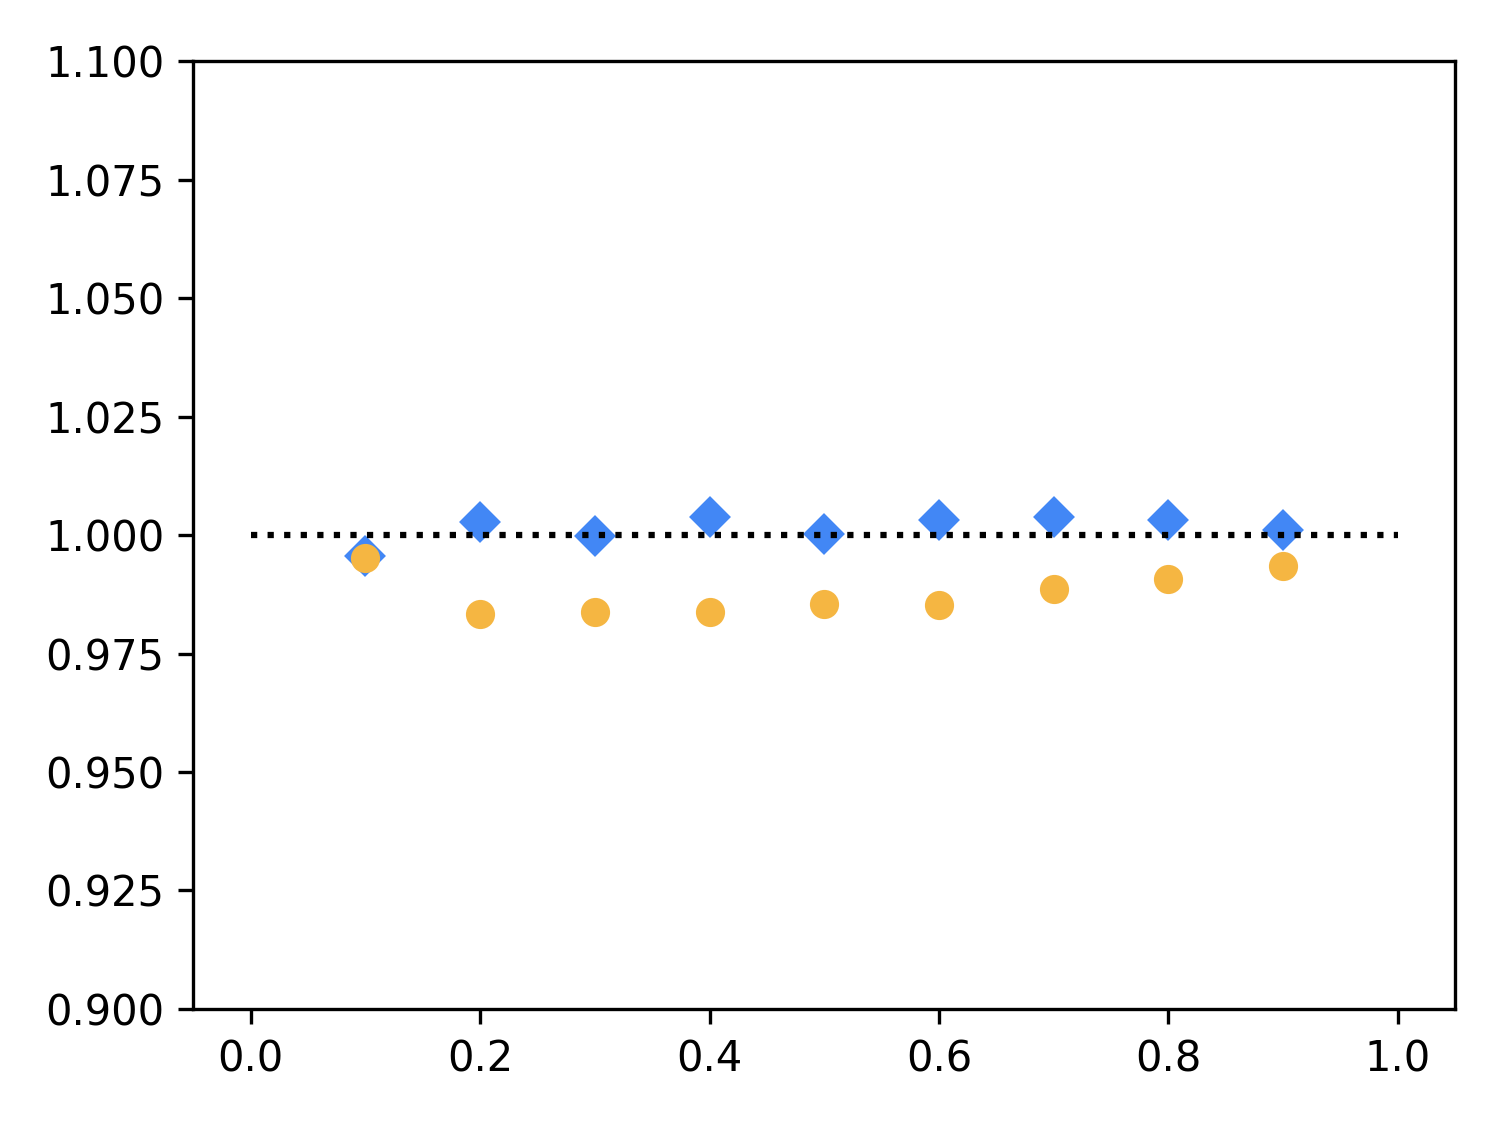
\includegraphics[width=0.9\columnwidth]{images/var_interval.png}
			\caption{Varianz Intervall: Verhältnis zwischen $\gamma$ (x-Achse) und dem tatsächlichen Anteil an korrekt geschätzten Intervallen (y-Achse) für $1000$ Durchläufe je $\gamma$ mit Stichprobenumfang $100$}
			\label{fig_var_interval_dot}
		\end{figure}
		

\section*{Ergebnisse und Diskussion}

\begin{thebibliography}{99}
	\bibitem{MathWorld}Weisstein, Eric W.: {\textit Buffon's Needle Problem.}, From MathWorld--A Wolfram Web Resource. \url{https://mathworld.wolfram.com/BuffonsNeedleProblem.html}
\end{thebibliography}

\end{document}